\section{Schematy różnicowe dla zadań dyfuzyjnych}

Będziemy korzystać z równania:

\[
\begin{cases}
\vspace{0.1cm} 
\hspace{0,1cm} \dfrac{\delta \psi}{\delta t} = D\dfrac{\delta^2 \psi}{\delta x^2} \hspace{1cm}, \Omega = [0,L]x[0,\infty] \\
\vspace{0.1cm}
\hspace{0,1cm}\psi_{(x,t)}|_{x=0} = 0 \hspace{0.8cm},t>0 \\
\vspace{0.1cm} 
\hspace{0,1cm}\psi_{(x,t)}|_{x=L} = 0 \hspace{0.7cm},t>0 \\
\vspace{0.1cm} 
\hspace{0,1cm}\psi_{(x,t)}|_{t=0} = \varphi(x) \hspace{0.3cm},x\in[0,L]
\end{cases}
\]

\subsection{Cel ćwiczenia}

Naszym zadaniem było stworzenie algorytmu rozwiązującego następujące równanie:

\[
\begin{cases}
\vspace{0.1cm} 
\hspace{0,1cm} \dfrac{\delta \psi}{\delta t} = D\dfrac{\delta^2 \psi}{\delta x^2} \\
\vspace{0.1cm}
\hspace{0,1cm}\psi|_{x=0} = 0 \\
\vspace{0.1cm} 
\hspace{0,1cm}\psi|_{x=L} = 0 \\
\vspace{0.1cm} 
\hspace{0,1cm}\psi|_{t=0} = sin(\frac{\pi x}{2})
\end{cases}
\]

, gdzie:

$\Omega = [0,2]x[0,1]$
\newline
$D=1$
\newline
\vspace{0.2cm}
$\psi_{analityczna}=\psi(x,t)=sin\Big(\dfrac{\pi x}{2}\Big)e^{-\Big(\dfrac{\pi^2 t}{4}\Big)}$

\subsection{Schemat FTCS}

FTCS (ang. Forward Time Central Space) czyli schemat "w przód":

$$\dfrac{\delta \psi}{\delta t} = D\dfrac{\delta^2 \psi}{\delta x^2}$$

Dla lewej strony równania zastosujemy schemat "w przód", natomiast dla prawej schemat centralny.

Mamy więc:

$$\dfrac{\psi^{(n+1)}_{i}-\psi^n_{i}}{\Delta t}=D\dfrac{\psi^{n}_{i+1}-2\psi^n_{i}+\psi^n_{i-1}}{\Delta x^2}$$

Stąd:

$$\psi^{(n+1)}_{i}=\dfrac{D\Delta t}{\Delta x^2}\Big(\psi^{n}_{i+1}-2\psi^{n}_{i}+\psi^{n}_{i-1}\Big)+\psi^{n}_{i} + O(\Delta t)+O(\Delta x^2)$$

Jest to schemat jawny, warunkowo stabilny, a więc parametry siatki muszą zostać dobrane we właściwy sposób.

Warunkiem stabilności dla takiego zadania jest następująca relcja:

$$\dfrac{D\Delta t}{\Delta x^2}\le \dfrac{1}{2}$$
\newpage
\subsection{Algorytm}

\begin{Shaded}
\begin{Highlighting}[]
\FunctionTok{clc}\NormalTok{,}\FunctionTok{clear} \FunctionTok{all}
\FunctionTok{tic}
\CommentTok{%rozwiązanie analityczne}
\NormalTok{G = @(x,t) }\FunctionTok{sin}\NormalTok{(}\BaseNTok{pi}\NormalTok{.*x./}\FloatTok{2}\NormalTok{).*}\FunctionTok{exp}\NormalTok{(-(}\BaseNTok{pi}\NormalTok{.^}\FloatTok{2}\NormalTok{).*t./}\FloatTok{4}\NormalTok{);}

\CommentTok{%przedział omega}
\NormalTok{xa=}\FloatTok{0}\NormalTok{;}
\NormalTok{xb=}\FloatTok{2}\NormalTok{;}
\NormalTok{yc=}\FloatTok{0}\NormalTok{;}
\NormalTok{yd=}\FloatTok{1}\NormalTok{;}

\CommentTok{%warunki brzegowe}
\NormalTok{u1 = @(x) }\FloatTok{0}\NormalTok{;}
\NormalTok{u2 = @(x) }\FloatTok{0}\NormalTok{;}
\NormalTok{u3 = @(x,t) }\FunctionTok{sin}\NormalTok{(}\BaseNTok{pi}\NormalTok{*x/}\FloatTok{2}\NormalTok{);}

\NormalTok{licznik=}\FloatTok{0}\NormalTok{;}
\CommentTok{%siatka}
\NormalTok{m=}\FloatTok{30}\NormalTok{;}
\NormalTok{D=}\FloatTok{1}\NormalTok{;}
\NormalTok{deltax=(xb-xa)/(m-}\FloatTok{1}\NormalTok{);}
\NormalTok{x=[xa:deltax:xb];         }\CommentTok{%przedział przestrzenny}
\NormalTok{deltat=(deltax^}\FloatTok{2}\NormalTok{)/(}\FloatTok{20}\NormalTok{*D); }\CommentTok{%dzielimy od razu przez 10, aby wartość }
\NormalTok{n_end=}\FunctionTok{floor}\NormalTok{(yd/deltat)+}\FloatTok{1}\NormalTok{; }\CommentTok{%nie była blisko deltat graniczne}
\NormalTok{t=[}\FloatTok{0}\NormalTok{:deltat:}\FloatTok{1}\NormalTok{];           }\CommentTok{%przedział czasowy}

\CommentTok{%macierz}
\FunctionTok{psi}\NormalTok{=}\FunctionTok{zeros}\NormalTok{(n_end,}\FunctionTok{length}\NormalTok{(x)); }\CommentTok{%utworzenie pustej macierzy}

\NormalTok{for }\BaseNTok{i}\NormalTok{=}\FloatTok{2}\NormalTok{:m-}\FloatTok{1}                \CommentTok{%dodanie warunku początkowego}
  \FunctionTok{psi}\NormalTok{(}\FloatTok{1}\NormalTok{,}\BaseNTok{i}\NormalTok{)=u3(x(}\BaseNTok{i}\NormalTok{));}
\NormalTok{end}
                        
\NormalTok{for n=}\FloatTok{2}\NormalTok{:n_end}
\NormalTok{  for }\BaseNTok{i}\NormalTok{=}\FloatTok{2}\NormalTok{:m-}\FloatTok{1}
    \FunctionTok{psi}\NormalTok{(n,}\BaseNTok{i}\NormalTok{)=(deltat/deltax^}\FloatTok{2}\NormalTok{)*(}\FunctionTok{psi}\NormalTok{(n-}\FloatTok{1}\NormalTok{,}\BaseNTok{i}\NormalTok{+}\FloatTok{1}\NormalTok{)-}\FloatTok{2}\NormalTok{*}\FunctionTok{psi}\NormalTok{(n-}\FloatTok{1}\NormalTok{,}\BaseNTok{i}\NormalTok{)+}\FunctionTok{psi}\NormalTok{(n-}\FloatTok{1}\NormalTok{,}\BaseNTok{i}\NormalTok{-}\FloatTok{1}\NormalTok{))+}\FunctionTok{psi}\NormalTok{(n-}\FloatTok{1}\NormalTok{,}\BaseNTok{i}\NormalTok{);}
\NormalTok{  end}
\NormalTok{  licznik = licznik+}\FloatTok{1}\NormalTok{;}
\NormalTok{end}

\NormalTok{[X,T] = }\FunctionTok{meshgrid}\NormalTok{(x,t);}
\FunctionTok{subplot}\NormalTok{(}\FloatTok{1}\NormalTok{,}\FloatTok{2}\NormalTok{,}\FloatTok{1}\NormalTok{)}
\FunctionTok{surf}\NormalTok{(X,T,}\FunctionTok{psi}\NormalTok{)}
\FunctionTok{title}\NormalTok{(}\StringTok{'Metoda Numeryczna'}\NormalTok{)}
\FunctionTok{subplot}\NormalTok{(}\FloatTok{1}\NormalTok{,}\FloatTok{2}\NormalTok{,}\FloatTok{2}\NormalTok{)}
\FunctionTok{surf}\NormalTok{(X,T,(G(X,T)))}
\FunctionTok{title}\NormalTok{(}\StringTok{'Metoda Analityczna'}\NormalTok{)}
\NormalTok{licznik}
\FunctionTok{toc}
\end{Highlighting}
\end{Shaded}
\newpage
\subsection{Wykresy}

Dla n = 5:

{\centering
	
	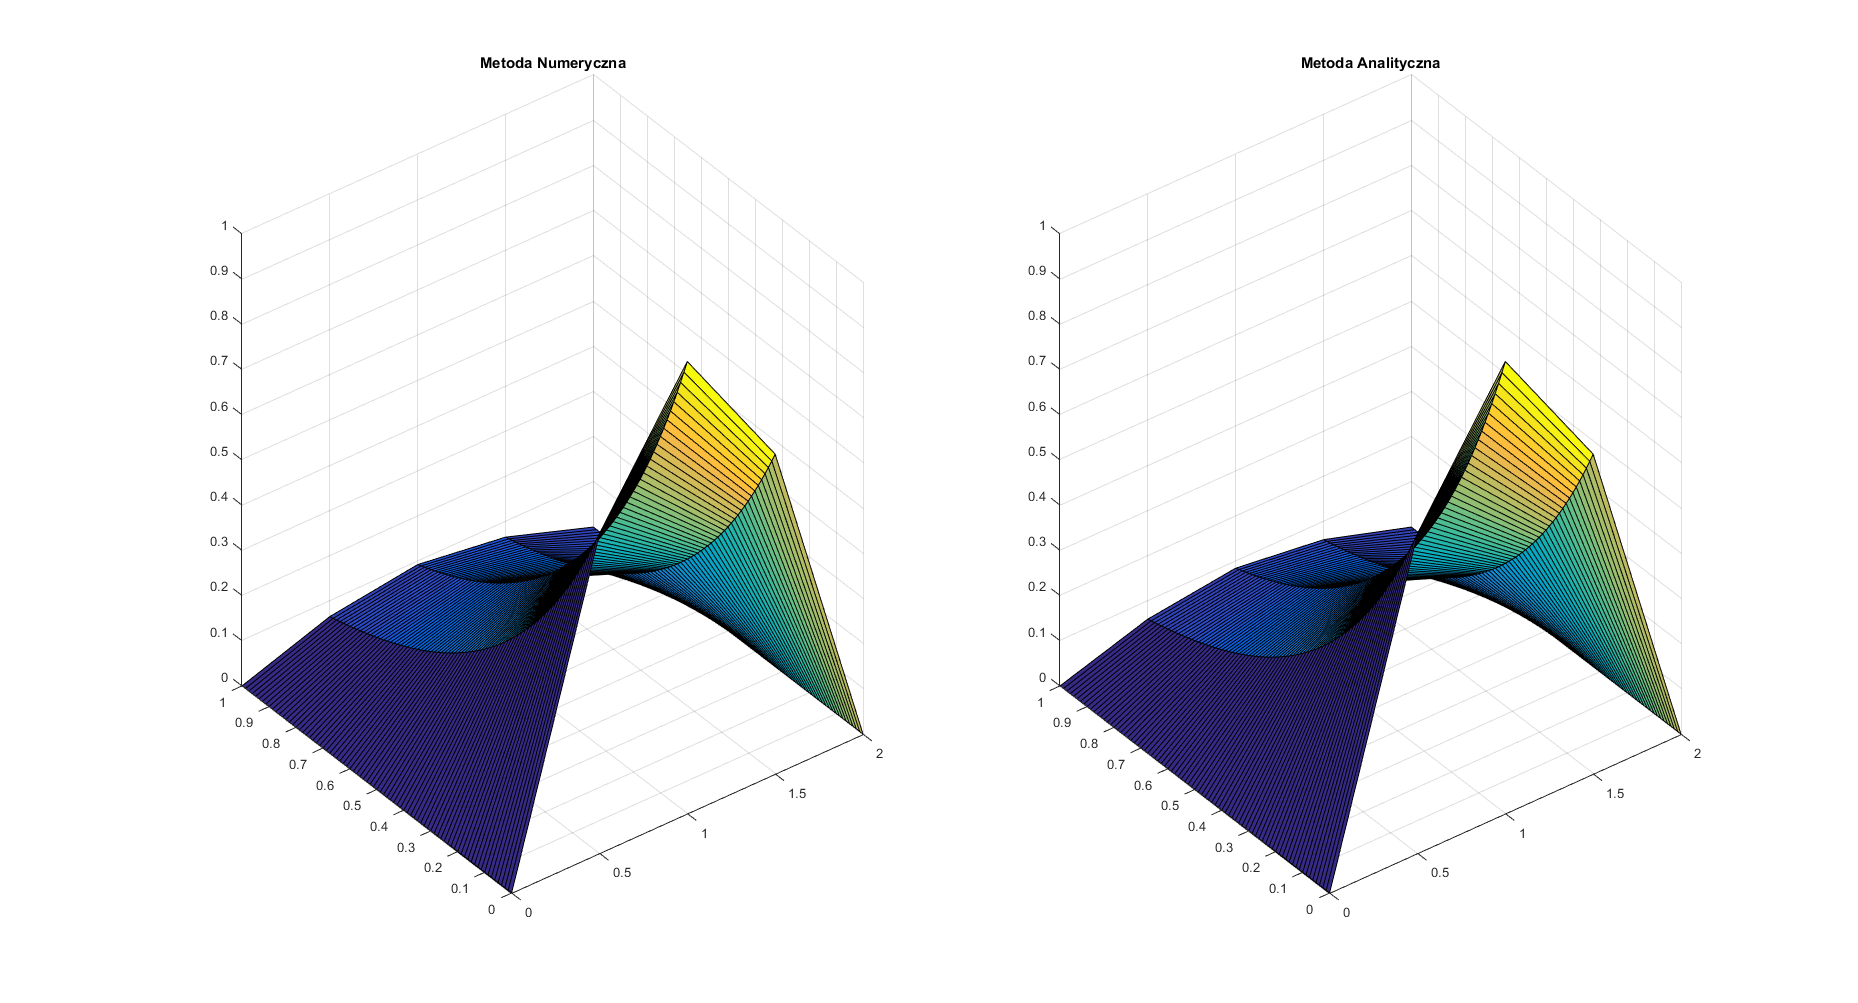
\includegraphics{Lab7/charts/ftcs/5.png}
	
}

Liczba wykonanych iteracji $ = 80 $

Czas wykonywania algorytmu $ = 0.100 s$

Dla n = 10:

{\centering
	
	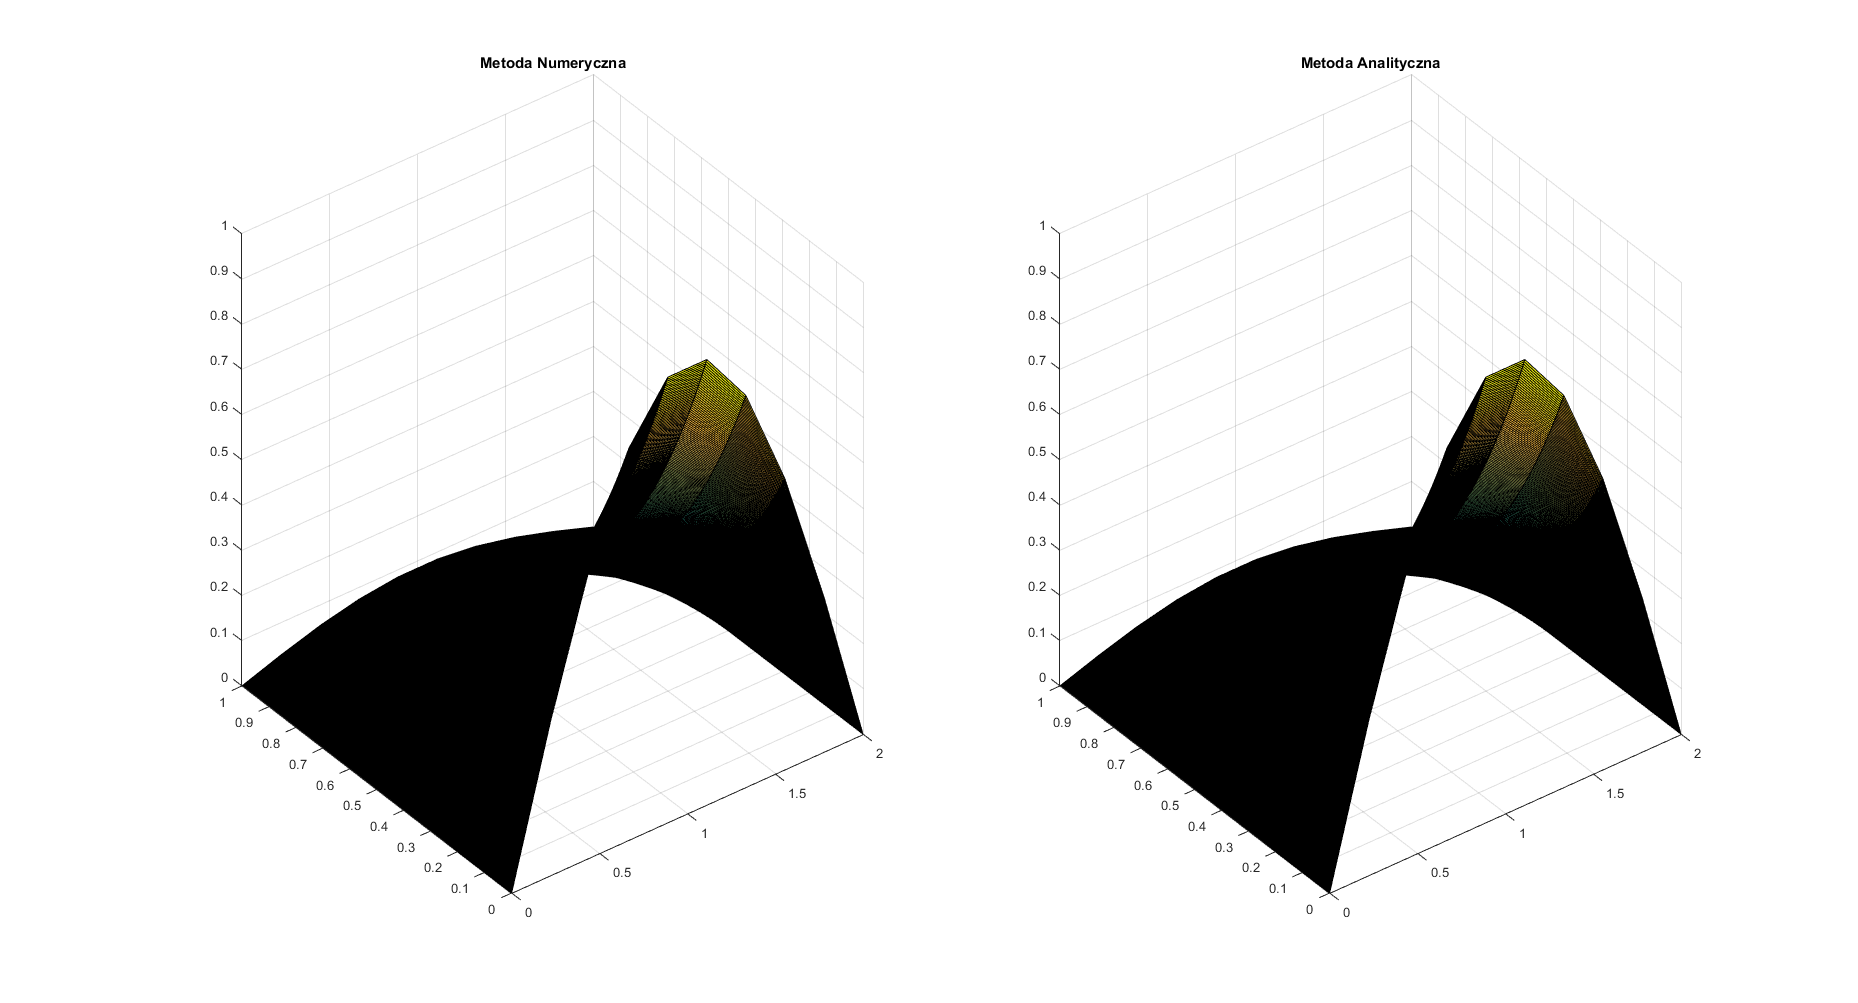
\includegraphics{Lab7/charts/ftcs/10.png}
	
}

Liczba wykonanych iteracji $ = 405 $

Czas wykonywania algorytmu $ = 0.163 s$

\newpage

Dla n = 15:

{\centering
	
	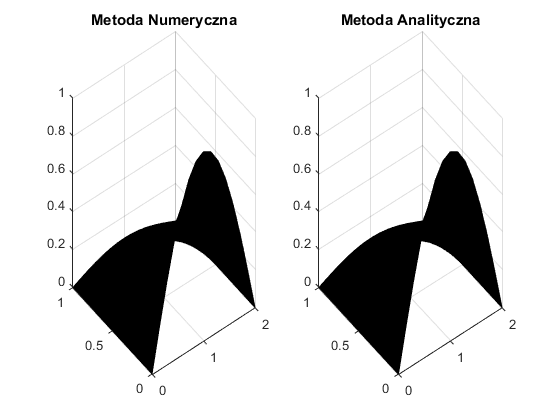
\includegraphics{Lab7/charts/ftcs/15.png}
	
}

Liczba wykonanych iteracji $ = 980 $

Czas wykonywania algorytmu $ = 0.192 s$

Dla n = 30:

{\centering
	
	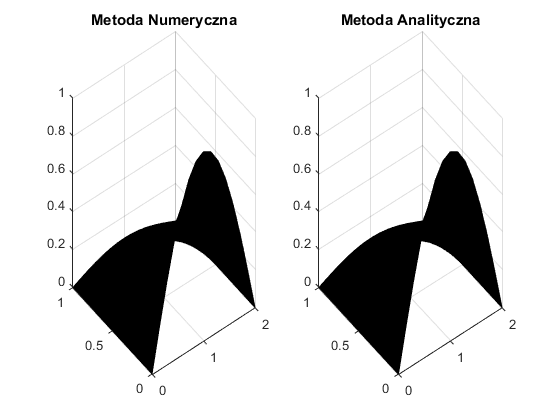
\includegraphics{Lab7/charts/ftcs/15.png}
	
}

Liczba wykonanych iteracji $ = 4205 $

Czas wykonywania algorytmu $ = 0.472 s$
\newpage
\subsection{Schemat BTCS}



